\documentclass[12pt,openany]{book}

% ---------- Fonts & encoding ----------
\usepackage[T1]{fontenc}
\usepackage[utf8]{inputenc}
\usepackage{XCharter}
\usepackage[scaled=0.90]{helvet}
\usepackage{microtype}

% ---------- Layout ----------
\usepackage[a4paper,inner=1.5in,outer=1.35in,top=1.35in,bottom=1.4in,headsep=20pt]{geometry}
\usepackage{xcolor}
\usepackage[most]{tcolorbox}
\usepackage{titlesec}
\usepackage{fancyhdr}
\usepackage{booktabs}
\usepackage{tikz}
\usetikzlibrary{arrows.meta,positioning,shapes.geometric,calc,fit,backgrounds}
\usepackage{lettrine}
\usepackage{enumitem}
\usepackage{graphicx}
\usepackage{parskip}
\usepackage[hidelinks]{hyperref}

% ---------- Brand palette (COMET) ----------
\definecolor{cometbrown}{HTML}{875503}
\definecolor{cometgold}{HTML}{C28119}
\definecolor{cometink}{HTML}{2B2B2B}
\definecolor{cometnavy}{HTML}{202080}
\definecolor{cometcream}{HTML}{FBF6EE}
\definecolor{cometrule}{HTML}{E4D9C6}
\definecolor{softgrey}{HTML}{6A6A6A}
\definecolor{cometgreen}{HTML}{2E7D32}

\color{cometink}

% ---------- Body spacing ----------
\setlength{\parskip}{0.6em}
\linespread{1.16}
\setlist{leftmargin=1.4em,itemsep=3pt,topsep=4pt}

% ---------- Headings ----------
\titleformat{\section}
  {\sffamily\bfseries\Large\color{cometbrown}}{}{0em}{}
\titleformat{\subsection}
  {\sffamily\bfseries\large\color{cometnavy}}{}{0em}{}
\titlespacing*{\section}{0pt}{1.9em}{0.55em}
\titlespacing*{\subsection}{0pt}{1.25em}{0.4em}

% ---------- Running heads ----------
\pagestyle{fancy}
\fancyhf{}
\renewcommand{\headrulewidth}{0pt}
\fancyhead[LE]{\sffamily\footnotesize\color{softgrey}\thepage\quad\textbullet\quad COMET}
\fancyhead[RO]{\sffamily\footnotesize\color{softgrey}Mapping Cerner to OMOP\quad\textbullet\quad\thepage}

% ---------- Callout boxes ----------
\newtcolorbox{definition}[1]{
  enhanced, breakable, colback=cometcream, colframe=cometgold,
  boxrule=0pt, leftrule=3pt, arc=2pt, left=10pt, right=10pt, top=8pt, bottom=8pt,
  fonttitle=\sffamily\bfseries\color{cometbrown}, title={#1}}
\newtcolorbox{practice}[1]{
  enhanced, breakable, colback=white, colframe=cometnavy,
  boxrule=0.6pt, arc=2pt, left=10pt, right=10pt, top=8pt, bottom=8pt,
  fonttitle=\sffamily\bfseries\color{cometnavy}, title={#1}}
\newtcolorbox{hood}[1]{
  enhanced, breakable, colback=black!3, colframe=black!35,
  boxrule=0pt, leftrule=3pt, arc=1pt, left=10pt, right=10pt, top=8pt, bottom=8pt,
  fonttitle=\ttfamily\bfseries\color{black!70}, title={#1}}

\newcommand{\pullquote}[1]{%
  \begin{center}\smallskip
  {\sffamily\itshape\large\color{cometbrown} #1}\smallskip\end{center}}
\newcommand{\code}[1]{{\ttfamily\small #1}}
\setcounter{secnumdepth}{0}

\begin{document}
\raggedbottom

% ============================================================
% HALF-TITLE
% ============================================================
\thispagestyle{empty}
\vspace*{3.5cm}
\begin{flushright}
{\sffamily\color{cometgold}\Large A CHAPTER IN CLINICAL DATA SCIENCE}\\[4pt]
{\color{cometrule}\rule{0.62\linewidth}{1.2pt}}
\end{flushright}
\vspace{2.2cm}
\begin{flushright}
{\sffamily\bfseries\fontsize{34}{40}\selectfont\color{cometink} From Bedside\\ to Benchmark}\\[14pt]
{\sffamily\Large\color{cometbrown} Turning a Hospital's Private Vocabulary\\ into the Common Language of Research}
\end{flushright}
\vfill
\begin{flushright}
{\itshape\color{softgrey} A working tour of terminology mapping, the OMOP Common\\
Data Model, and a tool called COMET.}
\end{flushright}
\clearpage

% ============================================================
% CHAPTER OPENER
% ============================================================
\thispagestyle{empty}
\begin{flushleft}
{\sffamily\bfseries\color{cometgold}\Large CHAPTER 7}\\[2pt]
{\color{cometrule}\rule{\linewidth}{2.5pt}}\\[10pt]
{\sffamily\bfseries\fontsize{27}{31}\selectfont\color{cometink} From Bedside to Benchmark}\\[12pt]
{\color{cometrule}\rule{\linewidth}{0.8pt}}
\end{flushleft}
\vspace{4pt}
{\itshape\color{softgrey} How a mapping tool takes the raw, idiosyncratic codes of an electronic
health record and translates them, term by term, into the standardized concepts that let
hospitals around the world ask the same question and trust the same answer.}
\vspace{8pt}
{\color{cometrule}\rule{\linewidth}{0.8pt}}
\vspace{2pt}

\lettrine[lines=3,lhang=0.15,findent=2pt,nindent=4pt]{\color{cometbrown}I}{magine} two hospitals, a
thousand kilometres apart, each trying to answer the same simple-sounding question: \emph{how many
of our patients with diabetes were prescribed a particular class of drug, and what happened to them?}
Both hospitals have the data. Both keep meticulous records of every diagnosis, every prescription,
every lab result. And yet, left to their own devices, they cannot combine their answers---because
although they are describing the same clinical reality, they are speaking different languages.

One hospital records ``diabetes'' as an internal numeric code that means nothing outside its own
database. The other uses a different code entirely. Their drug lists, their lab panels, their units of
measure---all locally defined, all subtly incompatible. This is the quiet, unglamorous obstacle at the
heart of modern health research: not a shortage of data, but a \emph{Babel} of it.

This chapter is about the bridge across that gap. We will first build up the two worlds that need
connecting---the world of the \textbf{electronic health record}, where clinical data is born, and the
world of the \textbf{OMOP Common Data Model}, where it can finally be shared. Then we will walk
through a working tool, \textbf{COMET}, that does the connecting: how it searches, how it guards
against mistakes, how a team of humans drives it, and how it turns thousands of small, careful
decisions into a single, trustworthy translation.

No prior knowledge of medical informatics is assumed. If you have ever wondered how a doctor's note
becomes a data point in a global study, read on.

\begin{practice}{In this chapter}
\textbf{Part I --- The Two Worlds.} The electronic health record and its private codes; the OMOP
Common Data Model and its shared concepts; the vocabulary tables that connect them; why mapping between
the two is genuinely hard; and the Canadian vocabularies that add a twist.\\[4pt]
\textbf{Part II --- The Tool at Work.} How COMET loads the vocabulary, imports source terms, and helps
a team map them---search, guardrails, precomputed candidates, review, drift control, and export---
followed by a single term's journey end to end, and the philosophy behind the design.
\end{practice}

\clearpage
% ============================================================
\section{Part I\quad The Two Worlds}
% ============================================================

\subsection{Where the data is born: the electronic health record}

Every time a clinician does something---admits a patient, records a diagnosis, orders a test,
prescribes a drug---a modern hospital writes it down electronically. The software that does this
writing is the \textbf{electronic health record}, or EHR. In much of North America, including at the
health authority this chapter draws its examples from, that software is \textbf{Cerner Millennium}
(now part of Oracle Health): a vast, decades-old clinical system that quietly underpins the daily work
of hundreds of hospitals.

An EHR is, at its core, an enormous and highly structured database. But it was built to \emph{run a
hospital}, not to \emph{answer research questions}, and that distinction shapes everything. To keep
data consistent, an EHR relies on \textbf{code sets}: controlled lists of allowed values. Rather than
let a nurse type ``Lions Gate Hospital'' as free text---and misspell it a dozen ways---the system
offers a dropdown backed by a numeric code. Every location, every encounter type, every kind of lab
result, every clinical event has such a code.

\begin{definition}{Source terminology}
The complete set of codes a hospital uses internally---its locations, its lab identifiers, its
diagnosis and procedure codes---is its \emph{source terminology}. Much of it is \emph{local}: invented
by, and meaningful only to, that one institution. A code like \code{2550791547} might mean ``Lions
Gate Hospital'' in one hospital's Cerner instance and nothing at all anywhere else.
\end{definition}

These codes are organized, in practice, into what the teams working with them call \textbf{MR
sheets}, short for \emph{MappingReport} sheets. Each sheet is one family of related codes---all the
locations, say, or all the event types, or all the diagnoses. A single sheet can hold tens of
thousands of distinct terms, and crucially, each term carries a \textbf{usage count}: how often it
actually appears in the live clinical data. That number matters enormously, as we will see: it is the
difference between a code used half a million times and one used twice, and it tells a mapping team
where to spend its attention.

\pullquote{An EHR is a superb instrument for running a hospital and a frustrating one for comparing
hospitals. Bridging that gap is the whole game.}

So we have our first world: rich, structured, clinically complete---and hopelessly private. Each
hospital's terminology is an island. To make the data comparable, we need a mainland: a shared
vocabulary that every island can map to.

\subsection{A common language: OMOP and the OHDSI vision}

That shared mainland exists. It is called the \textbf{OMOP Common Data Model} (CDM), and it is
maintained by a global open-science collaborative called \textbf{OHDSI}---the Observational Health
Data Sciences and Informatics program, pronounced ``Odyssey.''

The idea behind OMOP is deceptively simple. If every institution transforms its data into the
\emph{same} table structure, using the \emph{same} set of concepts to describe clinical facts, then a
piece of analysis written once can run \emph{anywhere}, unchanged. A researcher can develop a study on
their own data, publish the code, and have a dozen other institutions run the identical analysis on
their populations---each behind their own firewall, no raw patient data ever leaving the building.
Only the aggregate results are shared and compared. This is how OHDSI has powered studies spanning
hundreds of millions of patients across dozens of countries.

\begin{practice}{A word on the ``network study''}
The pay-off of a common data model is a mode of research that is otherwise almost impossible: the
distributed network study. Because every site's data looks the same, one analytic package runs at all
of them. Rare-disease cohorts that no single hospital could assemble become tractable when twenty
hospitals contribute in parallel---and patient privacy is preserved, because only counts and
coefficients travel, never records. The mapping work in this chapter is the unglamorous groundwork
that makes that possible.
\end{practice}

\subsection{The shape of the model: a few dozen tables}

The CDM defines a few dozen tables, each with a fixed, documented shape. A handful carry the bulk of
the clinical story, and every one of them works the same way: a row records that a \emph{person}
experienced a \emph{concept} at a \emph{time}. The concept is the key. It is what turns a row from a
private note into a comparable fact.

\begin{center}
\small\sffamily
\begin{tabular}{@{}ll@{}}
\toprule
\textbf{OMOP domain} & \textbf{lands in this CDM table} \\
\midrule
Condition (diagnoses, problems) & \code{CONDITION\_OCCURRENCE} \\
Drug (medications, vaccines) & \code{DRUG\_EXPOSURE} \\
Measurement (labs, vitals) & \code{MEASUREMENT} \\
Procedure (interventions) & \code{PROCEDURE\_OCCURRENCE} \\
Visit (encounters, admissions) & \code{VISIT\_OCCURRENCE} \\
Observation (everything else) & \code{OBSERVATION} \\
\bottomrule
\end{tabular}
\end{center}

Notice the middle column is decided \emph{by the concept}, not by the source system. A code's
\emph{domain}---which we will meet properly in a moment---is what routes it to the right table. Map a
diagnosis to a Condition concept and it flows into \code{CONDITION\_OCCURRENCE}; the ETL that
populates the CDM does not need to be told, because the vocabulary already knows. This is why the
vocabulary, not the table list, is the true heart of the model.

\subsection{The heart of it: standardized vocabularies and the CONCEPT table}

Here is the single most important idea in this chapter. In OMOP, \emph{every clinical fact points at
a concept}, and every concept lives in one enormous reference table called \code{CONCEPT}. Load it
into a database and it holds millions of rows: every disease in SNOMED CT, every lab test in LOINC,
every drug ingredient in RxNorm, every unit in UCUM, and much more---all in a single, uniform
structure.

Each row---each \emph{concept}---has a handful of fields that do a remarkable amount of work. It is
worth seeing one in full. Here is the concept for essential hypertension as it actually appears:

\begin{center}
\small\sffamily
\begin{tabular}{@{}ll@{}}
\toprule
\code{concept\_id} & \code{320128} \\
\code{concept\_name} & Essential hypertension \\
\code{domain\_id} & Condition \\
\code{vocabulary\_id} & SNOMED \\
\code{concept\_class\_id} & Clinical Finding \\
\code{standard\_concept} & \code{S} \quad\textrm{(standard)} \\
\code{concept\_code} & \code{59621000} \\
\code{valid\_start\_date} \ / \ \code{valid\_end\_date} & \code{2002-01-31} \ / \ \code{2099-12-31} \\
\bottomrule
\end{tabular}
\end{center}

Read those fields as a sentence. \emph{This is concept number 320128, called ``Essential
hypertension.'' It is a Condition, drawn from the SNOMED vocabulary, where its own code is 59621000.
It is a standard concept---the one the whole world analyzes conditions against---and it is currently
valid.} Every one of those facts will matter when we start mapping to it.

Two fields deserve special attention. The \code{domain\_id} is the router we just met: it decides
which CDM table the concept belongs in. And the \code{standard\_concept} flag is the linchpin of the
entire enterprise.

\begin{definition}{Standard vs.\ non-standard concepts}
OHDSI chooses, for each domain, \emph{one} vocabulary to be the ``standard'' that all analysis runs
against---SNOMED CT for conditions, RxNorm for drugs, LOINC for measurements. Concepts in those
vocabularies are marked \textbf{standard} (\code{standard\_concept = 'S'}). Everything else---an
ICD-10 diagnosis code, for instance---is a \emph{non-standard} \emph{source} concept: perfectly valid
for recording what was originally written, but not something you analyze against directly. The rule of
the road in CDM v5.4 is simple and strict: \textbf{a mapping's target must be a standard, valid
concept.} Map to a non-standard code and your data silently falls out of every standard analysis.
\end{definition}

\subsection{The vocabulary is more than one table}

\code{CONCEPT} is the centrepiece, but four companion tables make it usable, and COMET loads all of
them. Together they are what a mapping tool actually searches, reasons over, and depends on.

\begin{center}
\small\sffamily
\begin{tabular}{@{}ll@{}}
\toprule
\textbf{Table} & \textbf{What it holds} \\
\midrule
\code{CONCEPT} & the concepts themselves (the row we just read) \\
\code{CONCEPT\_SYNONYM} & alternate names, including other languages \\
\code{CONCEPT\_RELATIONSHIP} & typed links between concepts (``Maps to'', \ldots) \\
\code{CONCEPT\_ANCESTOR} & the hierarchy: which concepts contain which \\
\code{VOCABULARY} & the list of source vocabularies and their versions \\
\bottomrule
\end{tabular}
\end{center}

\code{CONCEPT\_SYNONYM} is why a search for ``heart attack'' can find the concept whose official name
is ``Myocardial infarction,'' and---importantly in a bilingual country---why a French label can find
an English concept. \code{CONCEPT\_ANCESTOR} encodes the hierarchy: it records that ``Essential
hypertension'' sits beneath ``Hypertensive disorder,'' which sits beneath ``Disorder of cardiovascular
system,'' and so on. That lets a mapper climb up or down to find exactly the right level of
granularity---the single most-used feature of professional mapping tools, and one COMET provides.
\code{VOCABULARY}, the smallest table, quietly carries the most operationally important fact of all:
which \emph{version} of the vocabularies you are holding.

\subsection{Relationships, ``Maps to,'' and the deliverable}

How do non-standard and standard concepts connect? Through \code{CONCEPT\_RELATIONSHIP}, which records
typed links between concept pairs. The most important relationship in the entire model is called,
plainly, \textbf{``Maps to.''} It is the arrow that carries a non-standard source code to its standard
equivalent. An ICD-10 code for essential hypertension ``Maps to'' the standard SNOMED concept for
essential hypertension; follow that arrow and you have turned a billing code into an analyzable fact.
Related links---``Concept replaced by,'' for a concept that has been superseded---let the vocabulary
describe its own evolution, and, as we will see, let COMET repair maps automatically when the world
changes.

\begin{center}
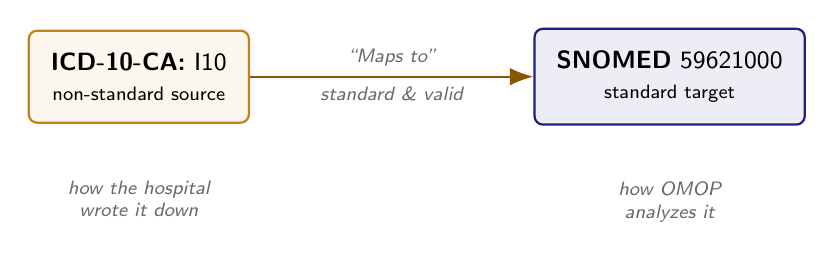
\begin{tikzpicture}[
  font=\sffamily\small,
  box/.style={rounded corners=3pt,draw,thick,align=center,inner sep=8pt,minimum height=2em},
  src/.style={box,fill=cometcream,draw=cometgold},
  std/.style={box,fill=cometnavy!8,draw=cometnavy},
  lbl/.style={font=\sffamily\scriptsize\itshape,color=softgrey}]
\node[src] (a) {\textbf{ICD-10-CA:} I10\\ \scriptsize non-standard source};
\node[std,right=3.6cm of a] (b) {\textbf{SNOMED} 59621000\\ \scriptsize standard target};
\draw[-{Latex[length=3mm]},thick,cometbrown] (a) -- node[above,lbl]{``Maps to''} node[below,lbl]{standard \& valid} (b);
\node[below=1.7em of a,lbl,align=center]{how the hospital\\ wrote it down};
\node[below=1.7em of b,lbl,align=center]{how OMOP\\ analyzes it};
\end{tikzpicture}
\end{center}

The output of all this mapping work has a canonical home. When you have decided that a particular
source code corresponds to a particular standard concept, you record that decision in a table called
\textbf{\code{SOURCE\_TO\_CONCEPT\_MAP}} (STCM for short). The STCM is, in a real sense, the
deliverable: a clean list of ``this local code means that standard concept,'' ready to drive the
extract-transform-load process that populates the CDM. Everything COMET does is, ultimately, in
service of producing a correct STCM.

\subsection{Why mapping is hard}

If mapping were merely ``look up the code and copy the answer,'' there would be no need for a chapter,
or a tool, or a team. It is hard for reasons worth naming, because each one shapes the design of
COMET.

\textbf{Ambiguity.} Source descriptions are terse, abbreviated, and written by busy clinicians. ``BP
sitting,'' ``Ca,'' ``Hx MI''---each could plausibly map to several concepts, and choosing correctly
needs clinical judgement, not string matching. Consider ``Ca'' alone: to a cardiologist it may suggest
\emph{cancer}; to a chemist, \emph{calcium}; in a lab-results sheet it almost certainly means the
serum-calcium measurement. The correct target depends on which sheet the term lives on, what the
neighbouring codes are, and sometimes a conversation with the clinician who created it. No algorithm
settles that; a knowledgeable human does. A good tool's job is to put the right evidence in front of
that human as fast as possible---which is exactly what the search, the usage count, and the
cross-references described later are for.

\textbf{Granularity and cardinality.} A local code may be broader or narrower than any single standard
concept. Sometimes one source term needs two target concepts; sometimes many source terms collapse to
one. There is rarely a tidy one-to-one correspondence.

\textbf{Scale and the long tail.} A single hospital can present a hundred thousand distinct codes. Most
appear rarely; a few appear millions of times. You cannot map everything by hand, so you must map
\emph{by impact}---highest-usage terms first---and this is exactly why that usage count travels with
every term.

\textbf{Drift and versioning.} The vocabulary is not frozen. Every quarter OHDSI publishes a new
release; concepts are retired, de-standardized, replaced. A mapping that was correct last year can be
silently broken by a concept that was deprecated in the interim. A serious tool must therefore treat
the vocabulary \emph{version} as a first-class fact and be able to re-check every existing map against
each new release.

\pullquote{Good mapping is not one hard decision. It is a hundred thousand small ones, made
consistently, revisited as the world changes.}

\subsection{The Canadian dimension}

The examples in this chapter come from a Canadian health authority, and Canada adds a genuine twist.
The international OMOP vocabularies do not include the classifications Canadian hospitals are required
to use. Those live with Canada's own standards bodies:

\begin{center}
\small\sffamily
\begin{tabular}{@{}lll@{}}
\toprule
\textbf{Vocabulary} & \textbf{Covers} & \textbf{Maintained by} \\
\midrule
ICD-10-CA & Diagnoses & CIHI \\
CCI & Interventions / procedures & CIHI \\
SNOMED CT-CA & Canadian-extension concepts & Infoway / SNOMED Int'l \\
pCLOCD & Lab observations (Canadian LOINC) & Infoway \\
DIN / DPD & Drug identifiers & Health Canada \\
\bottomrule
\end{tabular}
\end{center}

None of these are in the standard Athena download. So a Canadian mapping tool must be able to bring
them in as \textbf{custom source vocabularies}, following an OHDSI convention: custom concepts are
assigned identifiers in a reserved range---\code{concept\_id} at or above two billion---so they can
never collide with the official ones. Where a Canadian code has a genuine standard equivalent---and
CIHI helpfully publishes SNOMED\,CT-CA-to-classification maps that can seed exactly these
links---COMET records a ``Maps to'' relationship, and the Canadian code becomes analyzable. Where no
standard concept exists at all, we do something better than guessing: we \emph{flag it for the
standards body}. More on that shortly.

\clearpage
% ============================================================
\section{Part II\quad The Tool at Work}
% ============================================================

We now have both worlds and the gap between them. COMET---the Central Online Mapping and Export
Tool---lives in that gap. This half of the chapter follows the data through it, from an empty database
to a finished, exportable set of maps.

\begin{hood}{A note on the machinery}
COMET is a web application: a modern rebuild in the Laravel framework, backed by a PostgreSQL database
chosen precisely because it is the vocabulary's natural home in the OHDSI world. Mappers use it through
an ordinary browser. Nothing that follows requires you to think about that plumbing---but it is worth
knowing that the ``search'' and ``guardrail'' behaviours described below are real database queries
against a full copy of the OMOP vocabulary, not approximations.
\end{hood}

At a glance, the whole system is a pipeline with humans in the middle. Two streams flow in---the
standardized vocabulary from Athena, and the hospital's source terms from Cerner. They meet inside
COMET, where people map, review, and refine. And one clean stream flows out: the STCM that an ETL
turns into a populated CDM.

\begin{center}
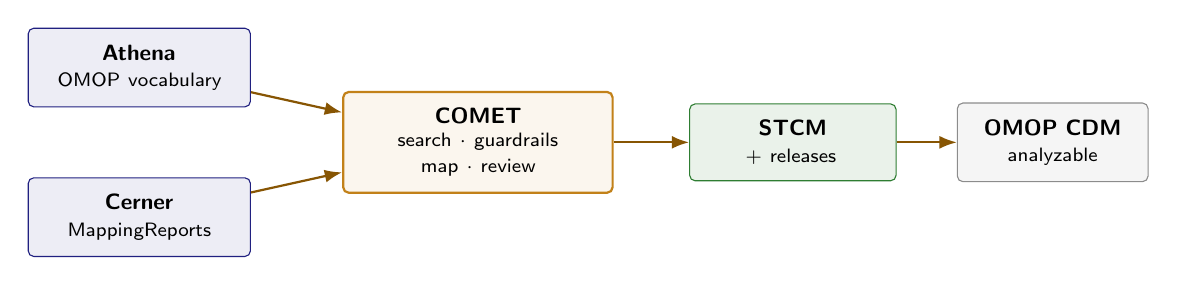
\begin{tikzpicture}[
  font=\sffamily\footnotesize,
  io/.style={rounded corners=2pt,draw,align=center,inner sep=6pt,minimum height=2.6em,text width=2.4cm},
  vin/.style={io,fill=cometnavy!8,draw=cometnavy},
  hub/.style={io,fill=cometcream,draw=cometgold,thick,text width=3cm,minimum height=3.4em},
  outbox/.style={io,fill=cometgreen!10,draw=cometgreen,text width=2.2cm},
  a/.style={-{Latex[length=2.2mm]},thick,cometbrown}]
\node[vin] (ath) at (0,0.95) {\textbf{Athena}\\ \scriptsize OMOP vocabulary};
\node[vin] (cer) at (0,-0.95) {\textbf{Cerner}\\ \scriptsize MappingReports};
\node[hub] (comet) at (4.3,0) {\textbf{COMET}\\ \scriptsize search $\cdot$ guardrails\\ \scriptsize map $\cdot$ review};
\node[outbox] (stcm) at (8.3,0) {\textbf{STCM}\\ \scriptsize + releases};
\node[io,fill=black!4,draw=black!45,text width=2cm] (cdm) at (11.6,0) {\textbf{OMOP CDM}\\ \scriptsize analyzable};
\draw[a] (ath) -- (comet); \draw[a] (cer) -- (comet);
\draw[a] (comet) -- (stcm); \draw[a] (stcm) -- (cdm);
\end{tikzpicture}
\end{center}

\begin{practice}{Where COMET sits in the OHDSI toolkit}
OHDSI already offers general tools for this work. \textbf{WhiteRabbit} scans a source database and
profiles its fields and value frequencies; \textbf{Usagi} suggests concept mappings by textual
similarity and lets a person review them. COMET occupies the same conceptual space as Usagi---
propose, then let a human decide---but is purpose-built for one institution's ongoing programme: it is
a shared web application rather than a desktop tool, it carries the review workflow, drift control,
Canadian vocabularies, and audit trail inside it, and it treats the usage counts and re-import cycle of
a live hospital as first-class. Think of it as Usagi's philosophy, industrialised for a team.
\end{practice}

\subsection{Step one: loading the vocabulary}

Before a single term can be mapped, COMET needs the mainland: a copy of the OMOP Standardized
Vocabularies. These are downloaded from OHDSI's \textbf{Athena} service---you choose which vocabularies
you need, and receive a set of large tab-delimited files---and loaded into COMET's database.

Loading is done carefully, because the vocabulary is both large and load-bearing. COMET stages the
incoming files into temporary tables, validates them, builds its search indexes, and only then swaps
the new vocabulary in for the old one in a single atomic operation. At no point does a mapper see a
half-loaded, inconsistent vocabulary. The moment the swap completes, the tool records \emph{which
release} it now holds, and that version stamp shows up throughout the interface---because, as we said,
knowing your vocabulary vintage is not optional.

\begin{practice}{Testing without the whole world}
A full Athena download is many gigabytes. To validate the pipeline you do not need all of it: a small,
real slice---a few administrative vocabularies, or a public teaching dataset---loads in seconds and
exercises every feature. COMET ships a one-command status report that, after any load, prints the
release, the concept counts per vocabulary, confirms the search indexes exist, and runs a live sample
query. ``Did it work?'' has a definite answer.
\end{practice}

\subsection{Step two: bringing in the source terms}

With the mainland in place, COMET imports the islands: the Cerner MappingReport extracts, one sheet at
a time. Each import is a substantial operation---a sheet can carry fifty thousand rows---so it runs as
a background job, and every run is recorded.

The import does something more interesting than a bulk insert. Because sheets are re-imported
periodically as the hospital's data evolves, COMET compares each incoming extract against what it
already holds and tracks \textbf{drift}: terms that are new in this report, terms still present, and
terms that have \emph{disappeared} since last time. A code that vanishes is not deleted---it is marked
``absent in latest MR,'' so its history and any mapping it carried are preserved while the mapper is
alerted that the clinical world has moved on. The extract also carries, for each term, a first-pass
suggested target and that all-important usage count, both of which flow straight into the mapping
screens.

\subsection{Step three: the act of mapping}

This is the centre of everything. A mapper opens a sheet and sees a grid: one row per source term, its
codes and description, its usage count, its status, and---if it has been mapped---its current target.
The unmapped rows are where the work is.

\textbf{Search that understands clinical language.} Click into a term and COMET offers candidate
concepts. Behind the innocuous search box sits a deliberately layered ranking engine, because plain
text matching is not good enough for clinical phrasing. It blends three signals: an \emph{exact code}
match, ranked first, always; \emph{trigram similarity}, which is robust to typos and word fragments
and---critically---accent-insensitive, so a French synonym matches an unaccented query; and
\emph{token coverage}, which catches long descriptions where the same words appear in a different
order. Among equally good matches, concepts the team \emph{already} maps to float upward, on the sound
assumption that consistency is usually right.

The effect is best seen in real output. The following are genuine top-ranked results, taken from
COMET running against a real slice of the OMOP vocabulary:

\begin{center}
\small\sffamily
\begin{tabular}{@{}lll@{}}
\toprule
\textbf{Mapper typed} & \textbf{Top concept returned} & \textbf{Why it matched} \\
\midrule
celecoxib & celecoxib (RxNorm) & exact name \\
Emphysema of lung & Pulmonary emphysema & re-ordered words \\
Brain, concussion & Concussion injury of brain & re-ordered words \\
House dust mite allergy & Allergy to house dust mite & re-ordered words \\
hemorrage stomach & Gastrointestinal hemorrhage & typo, via synonym \\
\bottomrule
\end{tabular}
\end{center}

Look at the middle three. A na\"ive search would miss every one, because the query words are present
but scrambled. The token-coverage signal is exactly what rescues them---and the last row shows the
engine shrugging off both a misspelling and a rephrasing to reach the right concept through a synonym.
This is the difference between a search box that frustrates mappers and one that earns their trust.

\pullquote{The search box is where a hospital's shorthand meets the world's standard vocabulary.
Everything upstream exists to make that meeting accurate.}

\textbf{Guardrails.} When a mapper chooses a target, COMET checks it against the CDM v5.4 rule before
saving. Try to map to a non-standard or retired concept and the tool refuses---but it does not merely
refuse. It reads the vocabulary's own ``Maps to'' and ``replaced by'' relationships and offers the
correct standard replacement as a one-click alternative. The rule that would otherwise be a source of
silent, downstream data loss becomes a helpful nudge at the moment of decision.

\textbf{Candidates, precomputed.} Searching live for every one of a hundred thousand terms would be
slow. So COMET can run its ranking engine in advance, across an entire sheet, and store the top
candidates for each unmapped term. When a mapper arrives at a term, the suggestions are already there,
instantly.

\begin{practice}{What ``precomputed'' looks like at scale}
Run against a real vocabulary, COMET's candidate engine produced \textbf{124{,}621} ranked suggestions
across \textbf{48{,}180} source terms in a single pass---so that not one of those terms costs a mapper
a wait. And to be unambiguous: this is \emph{not} auto-mapping. Nothing is ever written to a map
without a human confirming it. The machine lays out the options; the person decides.
\end{practice}

\textbf{Mapping mode.} For volume work, COMET offers a keyboard-driven queue that walks a sheet's
unmapped terms highest-usage-first, showing each term with its precomputed candidates. Number keys
accept a candidate; single letters set a status---exclude, question, escalate; another advances to the
next term. A skilled mapper can clear terms at a pace a mouse-driven form could never match, while
every action still passes through the same guardrails and is recorded in full.

\textbf{Equivalence and propagation.} A mapper can record \emph{how} exact a match is---equal, broader,
narrower, inexact---so downstream users know the fidelity of each link. And when the same description
has already been mapped elsewhere, COMET surfaces that decision and offers to apply it to every
identical unmapped term at once, turning a repeated judgement into a single click.

\begin{definition}{The three ways to say ``not a simple map''}
Not every term gets a standard concept, and COMET distinguishes three honest outcomes.
\textbf{Excluded}---the term is out of scope and should not be mapped at all. \textbf{Question}---the
mapper is unsure what the term means and needs a subject-matter expert; an \emph{internal} query.
\textbf{SDO Submission}---the term is real and mappable, but no standard concept for it \emph{exists
yet}. Rather than force a wrong target, the term is flagged for the relevant Standards Development
Organization (the OHDSI vocabulary team, or in Canada CIHI and Infoway). It joins an export queue, and
when the requested concept eventually ships in a future vocabulary release, the term becomes mappable
for real. This is the principled alternative to guessing.
\end{definition}

\subsection{A morning of mapping}

It helps to picture the work as a mapper actually experiences it. She signs in and her home screen
greets her with two things: a progress bar for the sheet she has been working---sixty-one percent
mapped, the number creeping up daily---and a short list, \emph{returned to you}, of three terms a
reviewer sent back yesterday with comments. She clears those first: one was mapped a shade too broadly,
and the reviewer's note points her to a more specific concept; two clicks and it is resolved and back
in the review queue.

Then she opens the sheet in mapping mode and settles into rhythm. The highest-usage unmapped term
appears with its candidates already ranked. \code{1}. Next. \code{1}. Next. A term she does not
recognise---some departmental abbreviation---she marks with \code{q}, a question for the clinical lead,
and moves on without breaking stride. Another has no plausible standard target at all; \code{s} sends
it to the standards-body queue. Every few minutes the little counter in the corner ticks up: fourteen
mapped this session, then twenty, then thirty. None of it feels like fighting the software, which is
the whole point. The tool's job is to disappear, leaving only the judgement.

\subsection{Step four: trust, but verify}

Mapping decisions are consequential, so COMET separates \emph{making} a map from \emph{approving} it.
Every change---every add, update, delete, and status change---is written to an immutable audit trail,
capturing who did what, when, and to which term, along with a snapshot of the source codes as they
stood at that moment.

A \textbf{reviewer} works a queue of pending changes. For each, they see a before-and-after: the
previously approved state beside the current one, and the list of pending edits. They can
\textbf{approve}---which stamps the change and records a new baseline snapshot---or \textbf{request
changes}, returning the term to its mapper with a required comment. A returned term surfaces on the
mapper's home screen; when they revise it, the flag clears and it flows back for approval. It is an
ordinary, humane editorial loop, and it is what turns a pile of individual guesses into a vetted,
defensible mapping.

\subsection{Step five: keeping current}

Recall that the vocabulary drifts. Every quarter brings a new Athena release, and some fraction of
existing maps will now point at concepts that have been deprecated or de-standardized. COMET's answer
is the \textbf{vocabulary impact report}: run after each vocabulary load, it finds every map whose
target is no longer standard, no longer valid, or gone entirely, and---using the vocabulary's own
successor relationships---proposes the replacement. A reviewer can remap with one click or send the
term back to the question queue. This single feature is the difference between a mapping that quietly
rots and one that stays correct across years of vocabulary evolution.

\subsection{Step six: working as a team}

Mapping a hospital is not a solo effort, so COMET is built for a team. Opening a term \textbf{claims}
it, so two mappers never unknowingly work the same code; the claim expires on its own so nothing gets
stuck. A \textbf{team dashboard} shows each mapper's throughput, the review backlog and its aging, and
the state of the various queues---questions outstanding, terms awaiting the standards bodies, claims in
flight. Managers can see where the work is flowing and where it is stalled, from ground truth rather
than guesswork.

\subsection{Step seven: the output}

Finally, the deliverable. COMET exports the completed maps as a valid \textbf{SOURCE\_TO\_CONCEPT\_MAP}
---the OMOP-native format an ETL consumes---as well as a richer interchange format that carries the
equivalence and provenance, and focused lists such as the exclusions and the standards-body submission
queue. Crucially, maps can be frozen into named, vocabulary-tagged \textbf{releases}: a reproducible
snapshot of exactly which maps existed, against exactly which vocabulary vintage. Months later, when
someone asks how a study's data was mapped, the answer is not a shrug---it is a specific, retrievable
release.

It is worth seeing what all this work distils down to. A single line of the exported
SOURCE\_TO\_CONCEPT\_MAP is unremarkable to look at---and that is the point. Every hard decision, every
review, every guardrail has collapsed into a plain, machine-readable statement of equivalence:

\begin{center}
\small\sffamily
\begin{tabular}{@{}ll@{}}
\toprule
\code{source\_code} & \code{2119541} \quad\textrm{\small(the hospital's own code)} \\
\code{source\_vocabulary\_id} & Cerner \\
\code{source\_code\_description} & Coronary arteriosclerosis \\
\code{target\_concept\_id} & \code{4110948} \quad\textrm{\small(standard SNOMED)} \\
\code{target\_vocabulary\_id} & SNOMED \\
\code{valid\_start\_date} \ / \ \code{valid\_end\_date} & \code{2020-01-01} \ / \ \code{2099-12-31} \\
\bottomrule
\end{tabular}
\end{center}

Multiply that one line by tens of thousands, hand the file to an ETL, and a hospital's private clinical
record becomes a standardized dataset a stranger can analyze correctly. That transformation---from the
first column to the fourth---is the entire purpose of the tool.

\clearpage
% ============================================================
\section{A Single Term's Journey}
% ============================================================

To make all of this concrete, follow one real term the whole way through.

A Cerner sheet contains the source description \textbf{``Coronary arteriosclerosis,''} used, let us
say, tens of thousands of times. It arrives through the import pipeline, unmapped, carrying its usage
count. Overnight, COMET's candidate engine runs across the sheet; when a mapper opens the term the
next morning, the top suggestion is already waiting: the standard SNOMED concept \emph{Coronary
arteriosclerosis}, matched exactly, with a secondary candidate (\emph{Coronary artery bypass graft})
offered just in case.

The mapper, in mapping mode, presses \code{1}. COMET checks the target: standard, valid---the guardrail
is satisfied, no replacement needed. The map is written; the action is stamped into the audit trail
with the mapper's name and a snapshot of the source codes; the term drops out of the unmapped queue
and the mapper advances to the next. Because ``Coronary arteriosclerosis'' appears identically on a few
other rows, COMET offered to propagate the decision, and with one more click those too are mapped.

Later, a reviewer opens the queue, sees the pending change against its (empty) prior baseline, agrees,
and approves; a snapshot is recorded. A quarter later, a new vocabulary release arrives. The impact
report checks this map among thousands of others: the target is still standard and valid, so nothing
is required. When the health authority finally cuts a release for its ETL team, this map---source
code, standard \code{concept\_id}, vocabulary vintage and all---appears in the exported
SOURCE\_TO\_CONCEPT\_MAP, one clean line among many, ready to help populate a CDM that a researcher
three provinces away can query without ever knowing this hospital's private codes existed.

\begin{center}
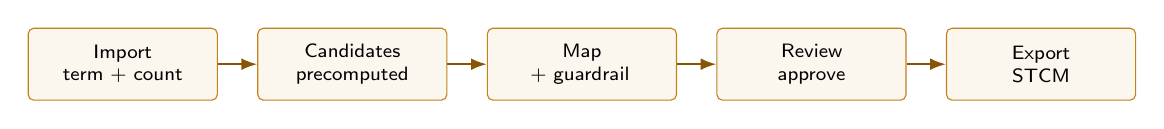
\begin{tikzpicture}[
  font=\sffamily\scriptsize,
  n/.style={rounded corners=2pt,draw,align=center,inner sep=5pt,fill=cometcream,draw=cometgold,minimum height=2.6em,text width=2.05cm},
  a/.style={-{Latex[length=2mm]},thick,cometbrown}]
\node[n](imp){Import\\ \scriptsize term + count};
\node[n,right=0.5cm of imp](cand){Candidates\\ \scriptsize precomputed};
\node[n,right=0.5cm of cand](map){Map\\ \scriptsize + guardrail};
\node[n,right=0.5cm of map](rev){Review\\ \scriptsize approve};
\node[n,right=0.5cm of rev](exp){Export\\ \scriptsize STCM};
\draw[a](imp)--(cand);\draw[a](cand)--(map);\draw[a](map)--(rev);\draw[a](rev)--(exp);
\end{tikzpicture}
\end{center}

\clearpage
% ============================================================
\section{Why It Is Built This Way}
% ============================================================

Step back from the mechanics and a design philosophy comes into focus. Three commitments run through
every part of COMET.

\textbf{The human decides; the machine assists.} At no point does COMET write a map on its own. Its
search, its precomputed candidates, its propagation---all of it accelerates human judgement without
replacing it. In a domain where a wrong map is worse than a missing one, because it corrupts silently,
this is not timidity; it is correctness.

\textbf{Correctness is enforced, not hoped for.} The standard-and-valid rule is not a guideline in a
manual that mappers are trusted to remember; it is a guardrail that fires at the moment of decision.
Drift is not something a team is expected to watch for; it is surfaced automatically after every
vocabulary release. The system makes the right thing the easy thing.

\textbf{Every decision is remembered.} The immutable audit trail, the review snapshots, the
vocabulary-tagged releases---together they mean that the answer to ``why is this term mapped this way,
and by whom, against which vocabulary'' is always available. In health data, where analyses inform
real decisions about real people, that provenance is not bureaucratic overhead. It is the foundation
of trust.

\pullquote{The goal was never to map faster than a human. It was to help a team of humans map
\emph{consistently}, \emph{correctly}, and \emph{accountably}---at a scale no human could manage
alone.}

The two hospitals from the opening can now, at last, answer their shared question together---not
because their data became identical, but because each, through patient work in a tool like this one,
learned to speak the common language while keeping its own. That translation, term by careful term, is
how the private record of a single bedside becomes part of the shared knowledge of medicine.

\vspace{1.2em}
{\color{cometrule}\rule{\linewidth}{0.8pt}}
\vspace{2pt}

{\sffamily\footnotesize\color{softgrey}
\textbf{Key terms in this chapter.}\quad
\textit{EHR} --- electronic health record, where clinical data is created.\;
\textit{Source terminology} --- a hospital's internal, often local, codes.\;
\textit{MR sheet} --- a Cerner MappingReport, one family of source codes.\;
\textit{OHDSI} --- the open collaborative behind OMOP.\;
\textit{OMOP CDM} --- the common data model that makes data comparable.\;
\textit{CONCEPT} --- OMOP's universal table of clinical concepts.\;
\textit{Domain} --- the kind of thing a concept is; it routes to a CDM table.\;
\textit{Standard concept} --- the one concept a domain is analyzed against.\;
\textit{Maps to} --- the relationship linking a source code to its standard target.\;
\textit{STCM} --- SOURCE\_TO\_CONCEPT\_MAP, the exported deliverable.\;
\textit{Athena} --- OHDSI's vocabulary download service.\;
\textit{SDO} --- a Standards Development Organization, to which genuinely unmappable terms are
escalated.}

\vspace{1.4em}
\begin{practice}{Where to go next}
The ideas in this chapter connect to a large and welcoming body of open work. The \emph{Book of
OHDSI} (freely available online) is the definitive, readable introduction to the Common Data Model and
its Standardized Vocabularies. The \textbf{Athena} website is where the vocabularies themselves are
browsed and downloaded. And the OHDSI community---forums, working groups, and an annual
symposium---maintains the standards, the tooling, and the collaborative studies that give all of this
mapping its purpose. A tool like COMET is one institution's contribution to that shared effort: the
careful, local work of translation that lets its data join the global conversation.
\end{practice}

\end{document}
